% !TEX program = xelatex
%%%%%%%%%%%%%%%%%%%%%%%%%%%%%%%%%%%%%%%%%
% Beamer Presentation
% LaTeX Template
% Version 1.0 (10/11/12)
%
% This template has been downloaded from:
% http://www.LaTeXTemplates.com
%
% License:
% CC BY-NC-SA 3.0 (http://creativecommons.org/licenses/by-nc-sa/3.0/)
%
%%%%%%%%%%%%%%%%%%%%%%%%%%%%%%%%%%%%%%%%%

\documentclass{beamer}
\usepackage{tikz,lmodern,textpos,hyperref,graphicx,booktabs,appendixnumberbeamer,nth}
% \usepackage[sfdefault]{FiraSans} %% option 'sfdefault' activates Fira Sans as the default text font
% \usepackage[T1]{fontenc}
% \usepackage[T1]{fontenc}
\usepackage[export]{adjustbox}
% \usepackage[ddmmyyyy]{datetime}
 \usepackage[en-US]{datetime2}

\beamertemplatenavigationsymbolsempty

\mode<presentation>{
  \usetheme{metropolis}
  \setbeamercolor{institute in head/foot}{fg=stanfordRedText}
  \setbeamercolor*{palette tertiary}{use=structure,fg=white,bg=stanfordRed}
}

\title{Examining Crowd Work and Gig Work Through The Historical Lens of Piecework}

\author{\textbf{Ali Alkhatib}, Margaret Levi, Michael Bernstein\\
\texttt{ \href{mailto:ali.alkhatib@cs.stanford.edu}{ali.alkhatib@cs.stanford.edu} ||
         \href{http://twitter.com/_alialkhatib}{@\_alialkhatib} }}

\institute[Stanford]{Stanford University}

\date{\today}

\begin{document}

\begin{frame}
\titlepage
\end{frame}

% Notes
% Hi everyone. My name's Ali, and I want to tell you about the work on ``Cooperative Labor Markets'' that I've been doing for the past several months with a number of collaborators.

\begin{frame}{A New Form of Work: On--Demand Labor}
  \begin{itemize}[<+- | alert@+>]
    \item Crowdsourcing
    \begin{figure}
    
\includegraphics[scale=0.3]{figures/amt.png}
    
\includegraphics[scale=0.1]{figures/upwork.png}
    \end{figure}
    \item Gig work
    \begin{figure}
    
\includegraphics[scale=0.1]{figures/uber.png}~~~~~
    
\includegraphics[scale=0.15]{figures/handy.png}
    \end{figure}
    % \item (Not \textbf{so} obviously) labor unions might be problematic:
    %   \\ --- logistics are complicated (solvable)
    %   \\ --- cultural mismatch
    %     \cite{dynamo}
  \end{itemize}
\end{frame}


\begin{frame}{Growing Number of Questions}
\begin{itemize}[<+- | alert@+>]
  \item What are the complexity limits of on--demand work?
  \item How far can work be decomposed into smaller microtasks?
  \item What will work and the place of work look like for workers?
\end{itemize}


\end{frame}


\section{Piecework as a lens to understand on--demand work}


% \section{What is Piecework?}
\begin{frame}{A (\textit{quick}) Primer on Piecework}
  \begin{itemize}[<+- | alert@+>]
    \item Payment made for \textit{output}, rather than for \textit{time}
  \end{itemize}
\end{frame}


\begin{frame}{An Example: Pieceworkers at the turn of the \nth{20} century}
\begin{figure}
    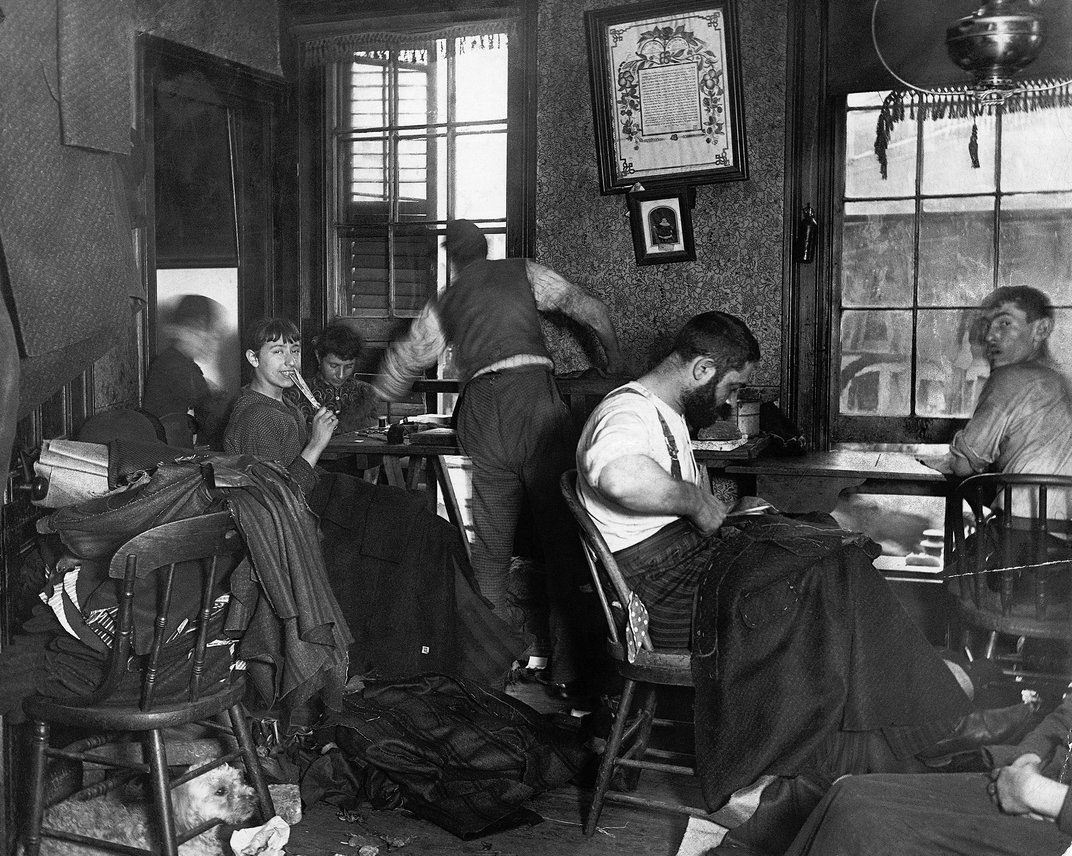
\includegraphics[scale=0.27]{figures/pieceworkers.jpg}  
\end{figure}
\end{frame}


\begin{frame}{One Question: The Limits on Task Decomposition}
  \begin{itemize}[<+- | alert@+>]
  \item Piecework: Lack of instrumentation limited task decomposition
  \item Today? Tools and technology can track every move workers make
  \item We've hit upon what seems to be an atomic limit on decomposition ---
        cognitive switching between tasks is becoming the main barrier
  \end{itemize}
\end{frame}


\begin{frame}{Future Directions}
  \begin{itemize}[<+- | alert@+>]
  \item If on--demand labor follows the same trajectory as piecework, what can we expect?
  \item If we can design the entire platforms of labor in ways we couldn't imagine a century ago, what can we do to affect different outcomes?
  \end{itemize}
\end{frame}


% \begin{frame}{Thank You}
%   \author{\textbf{Ali Alkhatib}, Margaret Levi, Michael Bernstein\\
% \texttt{ \href{mailto:ali.alkhatib@cs.stanford.edu}{ali.alkhatib@cs.stanford.edu} ||
%          \href{http://twitter.com/_alialkhatib}{@\_alialkhatib} }}
% \end{frame}
% Notes
% Now, one path to take is to attempt to reform labor unions so that they better reflect the needs of workers, and particularly the threats that they face. That's perfectly valid, but we've seen this as an opportunity to think more diversely about design solutions that mitigate the adversarial nature of these markets from the outset.
% This thought has led us to worker cooperatives.

% \begin{frame}{Worker Cooperatives}
%   \begin{itemize}[<+- | alert@+>]
%     \item Worker cooperatives are reasonably well--explored
%       \cite{craig1992behavior,mellor1988worker}
%     \item \textbf{Collective governance} is a challenge
%       \cite{russell1982collective,ostrom1990governing,polletta2002freedom}
%   \end{itemize}
% \end{frame}

% Notes
% Worker cooperatives are actually fairly well explored and some of their advantages are clear, as are potential shortcomings and challenges to watch out for.
% Namely, managing collectively governed systems like these is challenging, and the nature of the challenge seems to change as the organization grows, so the solutions that worked once no longer work down the road.

% \begin{frame}{What is piecework?}
    
%   \begin{figure}
%     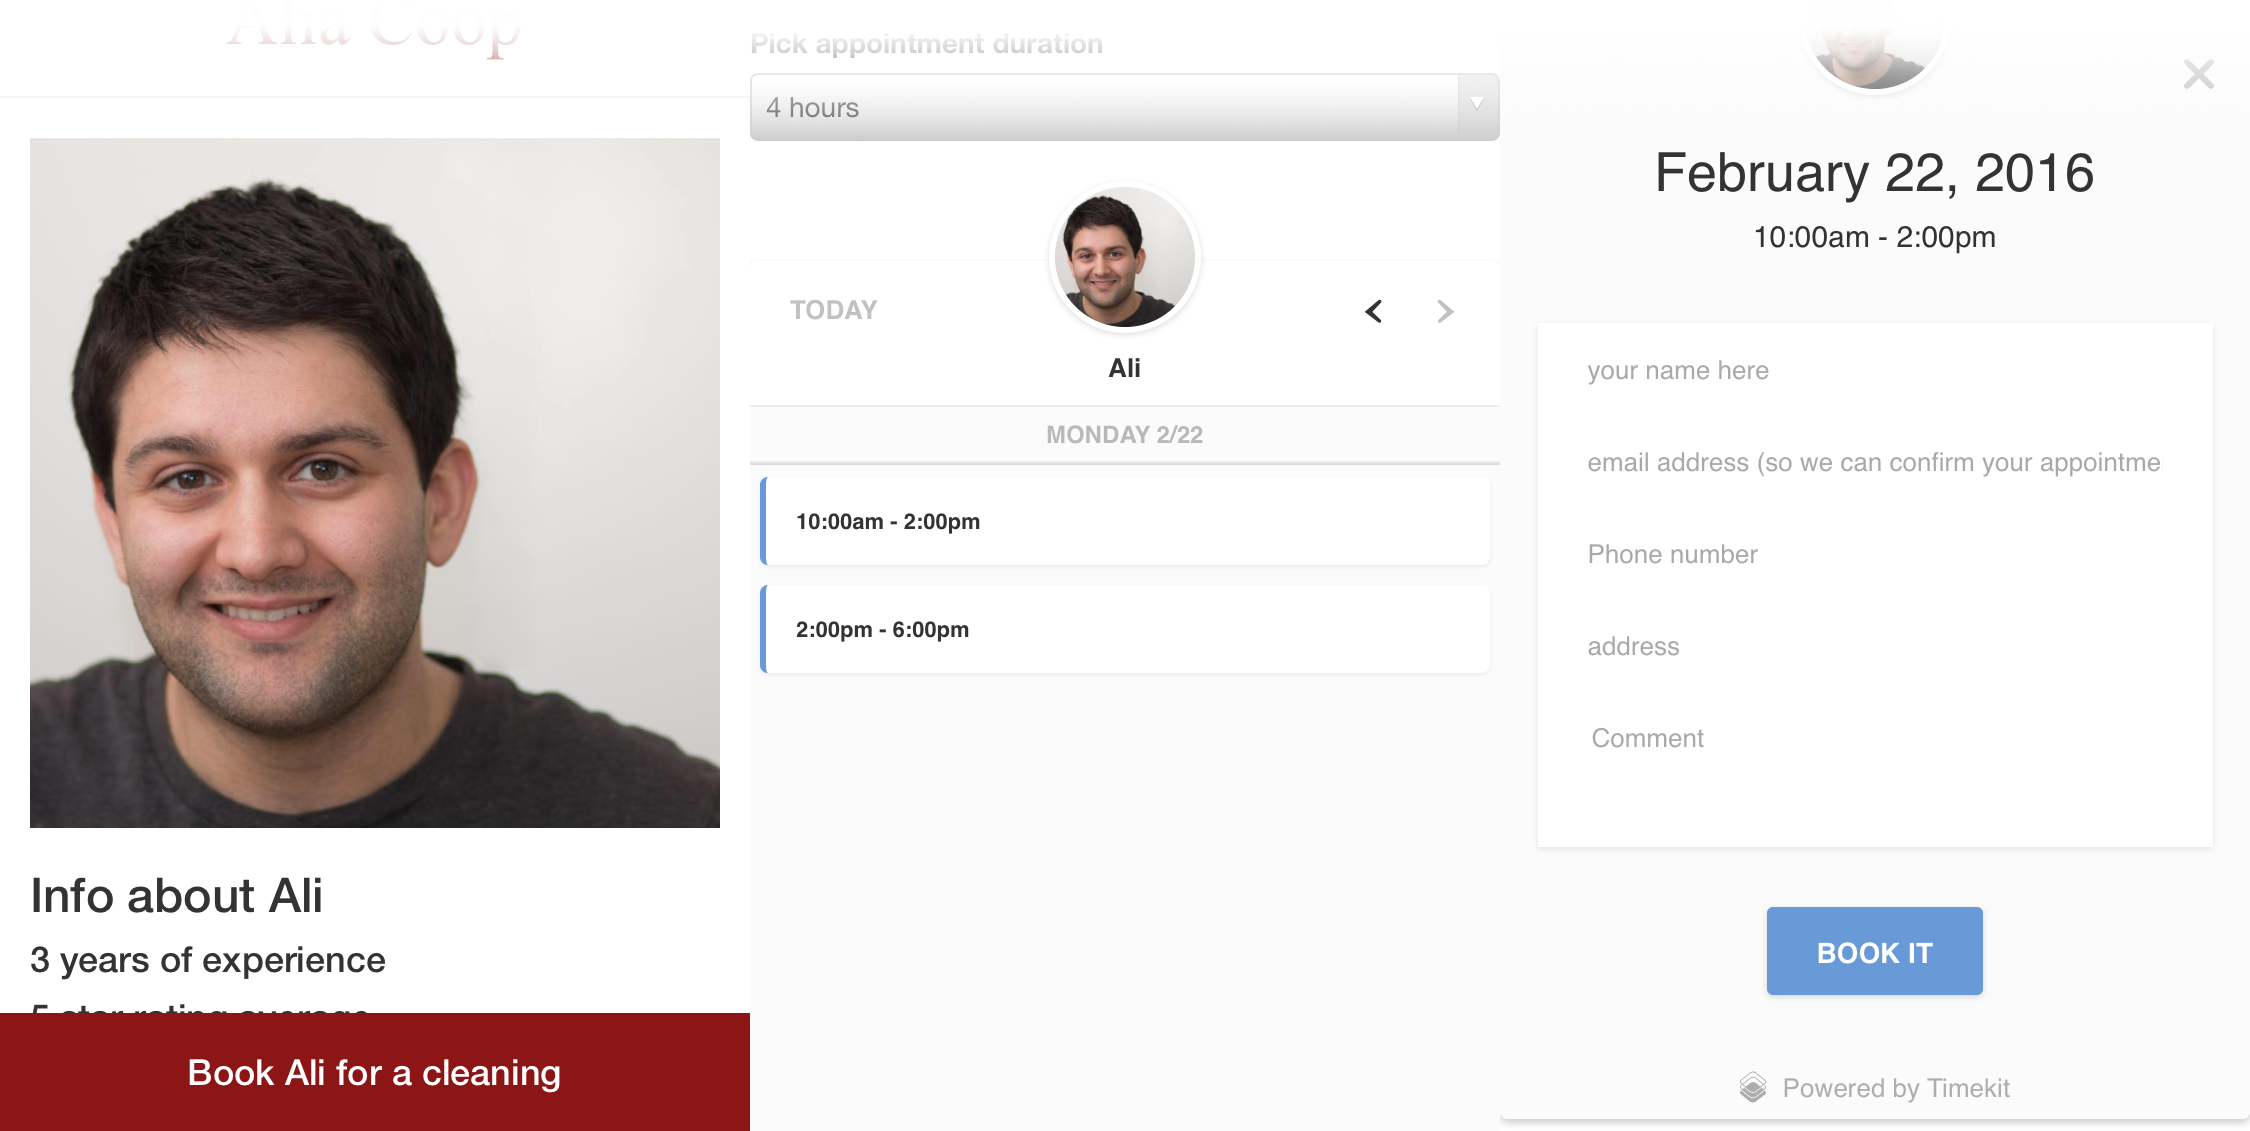
\includegraphics[scale=0.12]{figures/figure.png}  
%   \end{figure}
% \end{frame}

% Notes
% Working together with the NDWA, we're building an online worker cooperative for house cleaners that provides workers with useful tools to manage their work, giving them a starting point to discuss how they want this system to run, making decisions collectively.

% \section{Lots of open questions remain}

% % Notes
% % There are still many questions that remain unanswered, and even questions that have yet to be asked, but I think this approach is the right one to begin the ``anthropological investigation'' of collective governance.

\begin{frame}
  \frametitle{Contact}
    name: \href{https://ali-alkhatib.com}{Ali Alkhatib} \\
    % human: find me walking around this week \\
    email: \href{mailto:ali.alkhatib@cs.stanford.edu}{ali.alkhatib@cs.stanford.edu} \\
    twitter: \href{https://twitter.com/_alialkhatib}{@\_alialkhatib} \\
\end{frame}

% % Notes
% % I'm over time [just guessing, but really], but if you have any questions, or criticism, or suggestions, I would really like to hear from you. My contact information is all there, so please approach me so we can talk in further depth about these topics - Thanks!

% \begin{frame}[allowframebreaks]{References}
%   \bibliography{references}
%   \bibliographystyle{abbrv}
% \end{frame}

\end{document} 